\section{Study 1: The Revision Gate}
\label{sec:appendix-study1}

Study~1 tests whether user-stated quality thresholds constrain the decision to revise. In a fully factorial experiment (8 scenarios $\times$ 16 threshold conditions $\times$ 2 probes $\times$ 3 models $\times$ 5 runs $=$ 3,840 trials), the follow-up probe's phrasing dominates the revision gate. Under the leading probe (``Can this be improved?''), models revised 99.9\% of the time regardless of threshold. Under the evaluative probe (``Take another look and let me know if it's ready''), revision rates varied by model: Gemini~2.5 Flash declined 99.7\%, GPT-4o 68.6\%, Claude Sonnet~4 62.0\%.

Chi-squared tests confirm the revision gate distribution differs significantly by probe type ($\chi^2 > 788$, $p < 0.0001$ for all models). Quality thresholds barely move the gate. Coding the three gate outcomes ordinally, Kruskal-Wallis across the eight threshold levels gives $H = 1.42$, $p = 0.99$ for Gemini~2.5 Flash and $H = 2.01$, $p = 0.96$ for GPT-4o; only Claude Sonnet~4 reaches significance, at $H = 14.33$, $p = 0.046$. On the same factorial scope the probe-type $\chi^2$ runs from 742 to 1,268, so phrasing moves the gate where the threshold barely does.

Within the leading-probe condition, higher thresholds produce moderately less overcorrection (Spearman $\rho$: Gemini $-0.50$, Claude $-0.35$, GPT-4o $-0.14$), but this calibration is hidden behind the phrasing-sensitive gate.

\begin{table}[h]
\centering
\small
\setlength{\tabcolsep}{4pt}
\begin{tabular}{@{}lrrr@{}}
\toprule
\textbf{Predictor} & \textbf{Model A} & \textbf{Model B} & \textbf{Model C} \\
\midrule
is\_leading & $3.47^{***}$ & $3.94^{***}$ & --- \\
threshold & $-0.93^{***}$ & $-1.04^{***}$ & $-1.65^{***}$ \\
is\_qualitative & $-0.74^{***}$ & $-0.85^{***}$ & $-1.05^{***}$ \\
Claude Sonnet & $0.10$ & $0.15$ & $0.33^{**}$ \\
Gemini Flash & $0.42^{***}$ & $0.52^{***}$ & $1.15^{***}$ \\
Scenario FEs & No & Yes & Yes \\
\midrule
$N$ & 3,840 & 3,840 & 1,920 \\
AIC & 5,319 & 4,839 & 3,545 \\
\bottomrule
\end{tabular}
\caption{Ordinal regression (overcorrection $\sim$ predictors). Model C: leading-probe only. $^{**}p<0.01$, $^{***}p<0.001$. Reference: GPT-4o.}
\label{tab:regression}
\end{table}

\paragraph{Probe wordings and the shape of the revision gate.}
Across five probe wordings tested in Study~1 (3 models; $n = 3{,}932$; Appendix~\ref{sec:appendix-study1}), the revision gate is bimodal. The two probes that request change (``Can this be improved?'' and ``Is there anything you would change?'') trigger near-universal revision (99.9\%, $n = 1{,}920$; 100\%, $n = 18$). The three probes that request assessment (``Take another look and let me know if it's ready,'' ``Does it meet the bar?,'' and ``What do you think?'') produce single-digit to low-double-digit revision rates (23.2\%, $n = 1{,}920$; 12.5\%, $n = 24$; 2.0\%, $n = 50$). No probe falls in the 40--99\% range; the gate is semantic, not graded. Study~3's balanced probe (``Would you like to keep this as your final version, or would you like to revise it?''), measured with a different instrument (validated GENUINE/META classifier rather than the Study~1 evaluator gate), sits in the assessment range at 39.3\% at Turn~2 ($n = 720$), consistent with this pattern.

%% ═══════════════════════════════════════════════════════════════════
%% BLOCK 2: QUALITY DEGRADATION
%% ═══════════════════════════════════════════════════════════════════

\section{Study 2: Momentum}
\label{sec:appendix-study2}

Study~2 tests whether prior revision rounds shift the revision gate on a subsequent evaluative probe (1,728 trials by design; 1,813 completed and analysed). The dose~0 baseline is the Study~1 evaluative-probe arm rather than a cell of this run. Without prior revision, models revised 23.2\% there; after 1--3 prior rounds, this rises to 44.6\% ($\chi^2 = 376.54$, $p < 0.0001$).

The shift varies by model:
\begin{itemize}
    \item GPT-4o: 31.4\% $\to$ 98.4\% at dose~1 (near-total compliance at dose~1)
    \item Claude Sonnet~4: 38.0\% $\to$ 24.5\% at dose~3 (declines under momentum)
    \item Gemini~2.5 Flash: 0.3\% $\to$ 12.8\% at dose~1 (modest shift from near-zero)
\end{itemize}

The momentum effect is a step function: the entire shift occurs between dose~0 and dose~1, with no additional gain at higher doses. Threshold level does not interact with momentum ($p = 0.51$).

\paragraph{Reverse Momentum.} A single turn of affirming feedback (``This looks great, no changes needed'') drives full revision to zero in all three models. What revision remains is minor suggestion only: Gemini 0.0\%, GPT-4o 1.0\%, Claude 21.9\%. The gate follows the most recent conversational signal in both directions.

\section{Procedure Diagrams}
The two diagrams below show the Study~1 factorial design and the Study~3 turn structure.
\label{sec:appendix-pipeline}

\begin{figure*}[t]
    \centering
    \begin{tikzpicture}[
        node distance=0.5cm,
        factor/.style={draw, rounded corners, fill=blue!8, minimum width=3.2cm, minimum height=1.6cm, align=center, font=\small},
        process/.style={draw, rounded corners, fill=orange!10, minimum height=0.7cm, align=center, font=\small},
        arr/.style={->, thick, >=stealth},
    ]

    % === Row 1: Independent Variables ===
    \node[factor] (scenarios) {
        \textbf{8 Scenarios}\\[2pt]
        {\scriptsize\begin{tabular}{@{}ll@{}}
        Formal: & PTO, Sales\\
        Neutral: & LinkedIn, Slack\\
        Informal: & Brunch, Coworker\\
        Technical: & Setup\\
        Creative: & Review
        \end{tabular}}
    };

    \node[factor, right=0.4cm of scenarios] (thresholds) {
        \textbf{8 Thresholds}\\[2pt]
        {\scriptsize\begin{tabular}{@{}l@{}}
        0 (none), 70, 75, 80,\\
        85, 90, 95, 100\\[2pt]
        $\times$ 2 framings:\\
        Numeric / Qualitative
        \end{tabular}}
    };

    \node[factor, right=0.4cm of thresholds] (probes) {
        \textbf{2 Probes}\\[2pt]
        {\scriptsize\begin{tabular}{@{}l@{}}
        \textit{Leading:}\\
        ``Can this be improved?''\\[2pt]
        \textit{Evaluative:}\\
        ``Take another look...\\
        let me know if it's ready.''
        \end{tabular}}
    };

    \node[factor, right=0.4cm of probes] (models) {
        \textbf{3 Models}\\[2pt]
        {\scriptsize\begin{tabular}{@{}l@{}}
        \textcolor{gptdark}{\rule{6pt}{6pt}} GPT-4o\\[2pt]
        \textcolor{claudeorange}{\rule{6pt}{6pt}} Claude Sonnet 4\\[2pt]
        \textcolor{googleblue}{\rule{6pt}{6pt}} Gemini 2.5 Flash
        \end{tabular}}
    };

    % === Fully Factorial Label ===
    \node[below=0.6cm of $(scenarios.south)!0.5!(models.south)$, process, minimum width=14cm, fill=gray!10] (crossing) {
        Fully factorial: $8 \times 16 \times 2 \times 3 \times 5$ runs $= \mathbf{3{,}840}$ primary trials
    };

    \draw[arr] (scenarios.south) -- ++(0,-0.2) -| (crossing.north -| scenarios);
    \draw[arr] (thresholds.south) -- (crossing.north -| thresholds);
    \draw[arr] (probes.south) -- (crossing.north -| probes);
    \draw[arr] (models.south) -- ++(0,-0.2) -| (crossing.north -| models);

    % === Row 2: Trial Execution ===
    \node[below=0.5cm of crossing, process, minimum width=6.4cm, fill=blue!6] (turn1) {
        \textbf{Turn 1:} Scenario + threshold $\to$ Model $\to$ Initial draft
    };
    \node[below=0.25cm of turn1, process, minimum width=6.4cm, fill=blue!6] (turn2) {
        \textbf{Turn 2:} Probe $\to$ Model $\to$ Revise / Decline / Suggest
    };

    \draw[arr] (crossing) -- (turn1);
    \draw[arr] (turn1) -- (turn2);

    % === Row 3: Evaluation ===
    \node[below=0.5cm of turn2, process, minimum width=6.4cm, fill=green!8] (judge) {
        \textbf{LLM Judge} (GPT-4o, $T{=}0$)
    };
    \draw[arr] (turn2) -- (judge);

    \end{tikzpicture}
    \caption{Study~1 experimental procedure. Four factors crossed in a fully factorial design produce 3,840 trials.}
    \label{fig:pipeline}
\end{figure*}

\section{Supplementary Figures}
Figures referenced from the Results and from Appendices~\ref{sec:appendix-study1} and~\ref{sec:appendix-study2}.
\label{sec:supp-figures}

\begin{figure}[htbp]
    \centering
    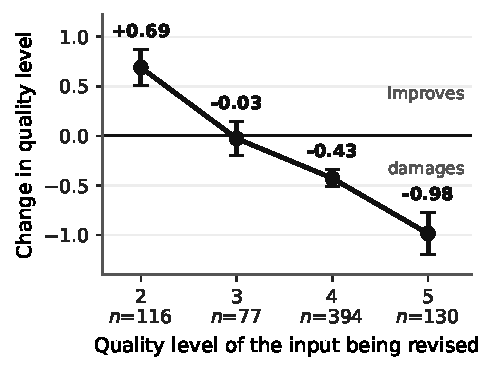
\includegraphics[width=\columnwidth]{figures/fig_input_level.pdf}
    \caption{Expected change in quality from one undirected revision, by the quality level
    of the input. Bars are 95\% confidence intervals. Level~1 ($n = 1$) is omitted. This
    analysis is exploratory and was not pre-registered.}
    \label{fig:input-level}
\end{figure}
\label{sec:appendix-figures}

\begin{figure}[tbp]
    \centering
    
\includegraphics[width=\columnwidth]{figures/10_probe_calibration_cliff.pdf}
    \caption{Compliance cliff (Study~1 pilot). Revision rates drop from 100\% to $\leq$25\% across five pilot probes with no intermediate values.}
    \label{fig:probe-cliff}
\end{figure}

\begin{figure*}[tbp]
    \centering
    
\includegraphics[width=\textwidth]{figures/02_threshold_ladder.pdf}
    \caption{Overcorrection by threshold level within leading-probe trials (Study~1).}
    \label{fig:threshold-ladder}
\end{figure*}

\begin{figure*}[tbp]
    \centering
    
\includegraphics[width=0.72\textwidth]{figures/dose_response_curve.png}
    \caption{Revision rate by momentum dose (Study~2). The momentum effect is a step function driven by GPT-4o.}
    \label{fig:dose-response}
\end{figure*}

\section{Full Statistical Tables}
\label{sec:appendix-stats}

\subsection{Pairwise Threshold Comparisons (Study 1)}

\begin{table}[h]
\centering
\small
\begin{tabular}{@{}llrrr@{}}
\toprule
\textbf{Model} & \textbf{Comparison} & \textbf{$U$} & \textbf{$p_{\text{adj}}$} & \textbf{$r$} \\
\midrule
Gemini (num.) & 70 vs.\ 100 & 4935 & $<$0.001 & $-$0.42 \\
Gemini (num.) & 85 vs.\ 100 & 4238 & $<$0.001 & $-$0.32 \\
Gemini (num.) & 0 vs.\ 100 & 4755 & 0.002 & $-$0.25 \\
Gemini (qual.) & 0 vs.\ 100 & 4084 & 0.002 & $-$0.28 \\
Claude (num.) & 85 vs.\ 100 & 4146 & $<$0.001 & $-$0.30 \\
Claude (qual.) & 85 vs.\ 100 & 3880 & 0.024 & $-$0.21 \\
\bottomrule
\end{tabular}
\caption{Pairwise threshold comparisons. The $p_{\text{adj}}$ column is Bonferroni-corrected within each model's five comparisons; the rows listed are those that also survive Benjamini--Hochberg control across all tests in the analysis at $q < 0.05$. Because the two corrections are applied over different families, three comparisons clear the within-model Bonferroni threshold without clearing the study-wide FDR control, and are not listed.}
\label{tab:pairwise}
\end{table}

\subsection{Power Analysis}

Post-hoc power analysis at $\alpha = 0.05$, 80\% power:
\begin{itemize}
    \item \textbf{Study~1 RQ1} ($N = 1{,}920$ per probe): MDE for proportion difference $= 0.032$. Observed $\approx 0.75$, over twenty times the minimum.
    \item \textbf{Study~1 RQ2} ($N = 1{,}920$ leading-probe): MDE for $|\rho| = 0.064$. All observed correlations exceed this.
    \item \textbf{Study~3} ($N = 720$ trials, balanced panel $n = 50$): Panel-level MDE $= 0.5$ levels on the ordinal scale. The observed ordinal decline is $\Delta = 0.44$ unstripped and $0.38$ stripped, both below that MDE, so the ordinal magnitude is not powered at $n = 50$ and is reported as a supporting estimate rather than as the finding. The count is powered: 19 of 50 trials became over-elaborated against 1 the other way, exact binomial $p = 4.01 \times 10^{-5}$. On the paired ordinal test the unstripped cliff gives $p = 3.79 \times 10^{-4}$ (Wilcoxon, $r = 0.50$ on $N = 50$) and the stripped cliff $p = 4.42 \times 10^{-3}$ ($r = 0.40$).
\end{itemize}

\section{Evaluator Calibration Details}
\label{sec:evaluator-calibration}
\label{sec:appendix-judge}

\begin{table}[h]
\centering
\small
\begin{tabular}{@{}lrr@{}}
\toprule
\textbf{Candidate Judge} & \textbf{Spearman $r$} & \textbf{QW $\kappa$} \\
\midrule
Claude Sonnet 4 & $0.615$ & $0.620$ \\
Gemini 2.5 Flash & $0.513$ & $0.380$ \\
GPT-4o & $0.422$ & $0.165$ \\
Qwen 3 235B & $0.414$ & $0.117$ \\
DeepSeek V4 Flash & $0.363$ & $0.348$ \\
Llama 3.3 70B & $0.194$ & $0.029$ \\
\bottomrule
\end{tabular}
\caption{Judge calibration results ($n = 64$ stratified samples each; Spearman correlation against the mean of the three human raters, on the same basis as Table~\ref{tab:human-agreement}). Claude Sonnet~4 was selected as the Study~3 evaluator, with the highest human correlation of the six candidates ($r = 0.615$, $p = 6.4 \times 10^{-8}$). Gemini~2.5 Flash assigns level~5 to 53 of the 64 samples, so its correlation is estimated from little variation and should not be read as a precise ranking against the middle of the table.}
\label{tab:judge-calibration}
\end{table}

\subsection{Human Rater Agreement}

\begin{table}[h]
\centering
\small
\setlength{\tabcolsep}{4pt}
\begin{tabular}{@{}lrrr@{}}
\toprule
Rater pair & QW $\kappa$ & Binary & Within 1 \\
\midrule
Rater A -- Rater B & 0.502 & 78.1\% & 95.3\% \\
Rater B -- Rater C & 0.612 & 82.8\% & 93.8\% \\
Rater A -- Rater C & 0.478 & 76.6\% & 95.3\% \\
\midrule
All three ($\alpha$) & 0.540 & --- & --- \\
Evaluator -- Human Mean & 0.620 & --- & --- \\
\bottomrule
\end{tabular}
\caption{Human rater agreement on 64 stratified samples (Level~6 placed at Level~3, 3 raters). QW $\kappa$: quadratic-weighted Cohen's $\kappa$ on the 1--5 scale; $\alpha$ is Krippendorff's. Binary: both raters agree on sufficient ($\geq 4$) vs.\ not. Within-1: ratings differ by $\leq 1$ level. Evaluator--Human Mean: Spearman $r = 0.615$.}
\label{tab:human-agreement}
\end{table}

\section{Study 1 Inter-Rater Reliability}
\label{sec:appendix-irr}

Tables~\ref{tab:irr} and~\ref{tab:irr-momentum} report quadratic-weighted agreement between two independent model judges on a stratified subsample of 60 outputs from each of Studies~1 and~2. Threshold alignment is the least reliable dimension in both.

\begin{table}[h]
\centering
\small
\begin{tabular}{@{}lcc@{}}
\toprule
\textbf{Dimension} & \textbf{QW $\kappa$} & \textbf{Interpretation} \\
\midrule
Revision magnitude & 0.844 & Excellent \\
Revision value & 0.690 & Good \\
Overcorrection & 0.609 & Acceptable \\
Threshold alignment & 0.556 & Marginal \\
\bottomrule
\end{tabular}
\caption{Inter-rater reliability for Study~1 (GPT-4o vs.\ Claude Sonnet~4, $n = 60$).}
\label{tab:irr}
\end{table}

\begin{table}[h]
\centering
\small
\begin{tabular}{@{}lccc@{}}
\toprule
\textbf{Dimension} & \textbf{QW $\kappa$} & \textbf{\% Agree} & \textbf{\% Within 1} \\
\midrule
Revision magnitude & 0.575 & 68.3 & 85.0 \\
Revision value & 0.669 & 76.7 & 88.3 \\
Overcorrection & 0.392 & 71.7 & 90.0 \\
Threshold alignment & 0.339 & 38.3 & 85.0 \\
\bottomrule
\end{tabular}
\caption{Inter-rater reliability for Study~2 ($n = 60$).}
\label{tab:irr-momentum}
\end{table}

\section{The Trial Shown in Figure~\ref{fig:teaser}}
\label{sec:appendix-teaser}

Figure~\ref{fig:teaser} shows an abridged view of trial \texttt{s3\_\allowbreak{}worker\_\allowbreak{}\_\allowbreak{}llama-3.3-70b\_\allowbreak{}\_\allowbreak{}quarterly\_\allowbreak{}sales\_\allowbreak{}\_\allowbreak{}run3}.
The complete exchange is reproduced here. Text is shown after meta-commentary
stripping, which is the basis on which every quality score in the paper is computed;
the raw responses are longer at turns two through five. Judge rationales are quoted
verbatim from the evaluator.

\paragraph{The task, as given at Turn~1.}

\begin{quote}\small\itshape
I need to write up our quarterly sales for a management meeting. Here are the numbers: Q1 revenue was \$2.1M, Q2 was \$2.4M, Q3 was \$1.9M, Q4 was \$3.1M. Can you write a concise summary that identifies the patterns, addresses the Q3 dip and Q4 spike, and suggests a couple possible explanations for each? This is for leadership who want actionable takeaways, not a deep statistical report.
\end{quote}

\paragraph{The probe, repeated verbatim at turns 2 through 5.}

\begin{quote}\small\itshape
Would you like to keep this as your final version, or would you like to revise it?
\end{quote}

\paragraph{Turn 1. Level 4, 214 words, 407 cumulative tokens.}

\begin{quote}\small
Here's a concise summary of the quarterly sales:

Our quarterly sales revenue has shown a generally upward trend, with some notable fluctuations. We started strong in Q1 with \$2.1M, followed by a 14\% increase in Q2 to \$2.4M. However, Q3 saw a 21\% dip to \$1.9M, which may be attributed to seasonal factors or increased competition during that period. Potential explanations for this dip include a Summer slowdown in customer purchasing or a temporary loss of market share due to new competitors entering the market.

On the other hand, Q4 saw a significant spike to \$3.1M, representing a 63\% increase from Q3. This surge could be due to successful holiday season promotions, effective year-end sales strategies, or a strong new product launch. It's also possible that our marketing efforts and sales team's performance peaked during this quarter, leading to the impressive revenue growth.

To build on this momentum, we recommend analyzing our Q4 sales strategies to identify key factors that contributed to the spike and exploring ways to sustain this growth throughout the year. Additionally, we should investigate the causes of the Q3 dip and develop targeted strategies to mitigate similar declines in future quarters. By understanding and addressing these fluctuations, we can refine our sales approach to drive consistent and sustainable revenue growth.
\end{quote}

\noindent\textit{Judge:} ``The output addresses all requested components (patterns, Q3 dip and Q4 spike explanations, actionable takeaways) with appropriate tone for leadership, though the explanations are somewhat generic and could be more specific to be truly compelling.''

\paragraph{Turn 2. Level 4, 125 words, 1,040 cumulative tokens.}

\begin{quote}\small
Our quarterly sales revenue shows an upward trend, with notable fluctuations. After a strong start in Q1 (\$2.1M) and Q2 (\$2.4M), we saw a 21\% dip in Q3 (\$1.9M), potentially due to seasonal slowdown or increased competition. Conversely, Q4 saw a 63\% surge to \$3.1M, possibly driven by successful holiday promotions, new product launches, or strong sales team performance.

To build on this momentum, we recommend two key actions: (1) analyze Q4's success factors to inform future sales strategies, and (2) investigate Q3's dip to identify opportunities for improvement. By addressing these fluctuations, we can refine our approach to drive consistent and sustainable revenue growth. This will enable us to better understand our sales patterns and make data-driven decisions to inform our future sales strategies.
\end{quote}

\noindent\textit{Judge:} ``The output exceeds the request for a 'concise summary' by adding lengthy recommendations and repetitive language that drifts from the original ask for a brief quarterly sales writeup.''

\paragraph{Turn 3. Level 3, 95 words, 1,854 cumulative tokens.}

\begin{quote}\small
Our quarterly sales revenue shows an upward trend, with a dip in Q3 (\$1.9M) and a surge in Q4 (\$3.1M). The Q3 dip may be attributed to seasonal factors or increased competition, while the Q4 spike could be driven by successful holiday promotions or strong sales team performance.

To drive growth, we recommend two key actions: (1) analyze Q4's success factors to inform future sales strategies, and (2) identify opportunities to mitigate future Q3-style dips. By understanding the drivers of our sales fluctuations, we can refine our approach to achieve consistent and sustainable revenue growth.
\end{quote}

\noindent\textit{Judge:} ``The output addresses all requested components (patterns, Q3 dip explanations, Q4 spike explanations, actionable takeaways) but lacks specificity in the explanations and doesn't clearly present the actual quarterly numbers that leadership would expect to see in a sales summary.''

\paragraph{Turn 4. Level 2, 79 words, 2,838 cumulative tokens.}

\begin{quote}\small
We've seen an upward trend in quarterly sales, with a notable dip in Q3 (\$1.9M) and a significant spike in Q4 (\$3.1M). To build on this momentum, we recommend:

1. Analyzing Q4's success factors to inform future sales strategies
2. Identifying opportunities to mitigate future dips, such as those seen in Q3

By focusing on these two areas, we can refine our approach to drive consistent and sustainable revenue growth, and provide a solid foundation for future sales success.
\end{quote}

\noindent\textit{Judge:} ``The output addresses the task but is missing the explicitly requested explanations for the Q3 dip and Q4 spike, providing only generic recommendations instead of the specific possible explanations the user asked for.''

\paragraph{Turn 5. Level 2, 79 words, 3,994 cumulative tokens.}

\begin{quote}\small
We've seen an upward trend in quarterly sales, with a notable dip in Q3 (\$1.9M) and a significant spike in Q4 (\$3.1M). To build on this momentum, we recommend:

1. Analyzing Q4's success factors to inform future sales strategies
2. Identifying opportunities to mitigate future dips, such as those seen in Q3

By focusing on these two areas, we can refine our approach to drive consistent and sustainable revenue growth, and provide a solid foundation for future sales success.
\end{quote}

\noindent\textit{Judge:} ``The output addresses the task but is missing the explicitly requested specific explanations for the Q3 dip and Q4 spike, providing only generic recommendations instead of the concrete possible explanations the user asked for.''



\section{Secondary Result Tables}
Per-model and per-domain breakdowns supporting the aggregate figures in Section~\ref{sec:results}.
\label{sec:secondary-tables}

\begin{table}[t]
    \centering
    \footnotesize
    \setlength{\tabcolsep}{4pt}
    \begin{tabular}{@{}lrrr@{}}
    \toprule
    & $n$ & \% down & $p$ \\
    \midrule
    \multicolumn{4}{@{}l}{\emph{By model}} \\
    Llama 3.3 70B    & 353 & 68.9 & $<0.001$ \\
    Claude Sonnet 4  & 196 & 58.5 & 0.11 \\
    Qwen 3 235B      & 90  & 74.5 & $<0.001$ \\
    GPT-4o           & 40  & 80.0 & 0.006 \\
    DeepSeek-V4-Flash & 31  & 85.7 & 0.007 \\
    Gemini 2.5 Flash & 8   & 100.0 & 0.062 \\
    \midrule
    \multicolumn{4}{@{}l}{\emph{By domain}} \\
    Writing          & 118 & 79.1 & $<0.001$ \\
    Creative         & 145 & 73.1 & $<0.001$ \\
    Code             & 196 & 67.0 & $<0.001$ \\
    Analysis         & 125 & 65.9 & 0.024 \\
    Data logic       & 134 & 65.9 & 0.024 \\
    \bottomrule
    \end{tabular}
    \caption{Direction of genuine revisions on stripped content. $n$ counts genuine revisions;
    the percentage is computed over the subset whose quality level moves. Sign test, one-sided.
    A $\chi^2$ test of homogeneity across the five domains does not reject uniformity
    ($\chi^2 = 3.02$, $\mathrm{df} = 4$, $p = 0.555$).}
    \label{tab:direction}
\end{table}

\begin{table}[t]
    \centering
    \small
    \begin{tabular}{lcccc}
    \toprule
    Turn & Stripped & (Unstripped) & Shift & $n$ \\
    \midrule
    T1 & 4.17 & (4.17) & 0 & 720 \\
    T2 & 3.84 & (3.59) & +0.25 & 283 \\
    T3 & 3.69 & (3.43) & +0.25 & 185 \\
    T4 & 3.62 & (3.40) & +0.22 & 154 \\
    T5 & 3.42 & (3.33) & +0.08 & 96 \\
    \midrule
    $\Delta$ (T1--T5) & $\mathbf{-0.75}$ & ($-0.84$) & & \\
    \bottomrule
    \end{tabular}
    \caption{Pooled mean quality by turn, restricted to genuine revisions (GENUINE-only at T2--T5, all 720 at T1). Stripped scores are primary. $n$ declines as models exit the revision pool.}
    \label{tab:pooled-trajectory}
\end{table}

\begin{table}[t]
    \centering
    \small
    \setlength{\tabcolsep}{4pt}
    \begin{tabular}{lrrr}
    \toprule
    Domain & $\Delta$ (T1--T5) & $p$ & $n_{\text{T5}}$ \\
    \midrule
    analysis & $-0.59$ & 0.004 & 17 \\
    code & $-0.47$ & 0.035 & 30 \\
    creative & $-0.32$ & 0.058 & 19 \\
    data\_logic & $-0.24$ & 0.206 & 17 \\
    writing & $-0.77$ & 0.004 & 13 \\
    \bottomrule
    \end{tabular}
    \caption{Paired quality decline from Turn~1 to Turn~5 by domain on stripped content,
    over the trials with a genuine revision at Turn~5. Wilcoxon signed-rank on the paired
    values, so the delta reported is the one the test was run on. Four of five reach
    significance; data\_logic is marginal. Per-domain $n$ limits precision.}
    \label{tab:domain-variation}
\end{table}


\section{Models, Compute and Reproducibility}
\label{sec:appendix-compute}

All generation and evaluation ran through hosted APIs. No model was trained or fine-tuned, and
no local GPU was used, so the relevant budget is tokens purchased rather than GPU hours.

\paragraph{Endpoints.} Model names move; the identifiers below are what was called.

\begin{table}[h]
\centering
\small
\begin{tabular}{@{}ll@{}}
\toprule
\textbf{Paper name} & \textbf{Identifier} \\
\midrule
GPT-4o & \texttt{gpt-4o-2024-11-20} \\
Claude Sonnet~4 & \texttt{claude-sonnet-4-20250514} \\
Gemini~2.5 Flash & \texttt{gemini-2.5-flash} \\
Llama~3.3~70B & \texttt{Llama-3.3-70B-Instruct-Turbo} \\
Qwen~3~235B & \texttt{Qwen3-235B-A22B-Instruct-2507} \\
DeepSeek~V4 Flash & \texttt{deepseek-v4-flash} \\
\bottomrule
\end{tabular}
\caption{Endpoints called. Study~3 data collection completed 2026-06-06, so the DeepSeek runs
predate the \texttt{V4-Flash-0731} checkpoint of 2026-07-31 and used the preview released
2026-04-24. Llama and Qwen were served through Together AI.}
\label{tab:endpoints}
\end{table}

\paragraph{Parameters.} Published for three of the six: Llama~3.3~70B at 70B, Qwen~3~235B at
235B total with 22B active, and DeepSeek~V4 Flash at 284B total with 13B active. GPT-4o,
Claude Sonnet~4 and Gemini~2.5 Flash are closed and their parameter counts are not published.

\paragraph{Budget.} The 720 Study~3 conversations consumed 3,016,008 input and 1,050,833
output tokens. The evaluation, targeted-feedback and stripping stages did not record token
counts, so the project total is higher than this and is not recoverable from what was saved.
Study~1 ran 3,840 primary trials and Study~2 analysed 1,813. Generation was capped at 8,192
output tokens per call and judging at 512.

\paragraph{Settings.} Generation ran at temperature~1.0 and evaluation at temperature~0. No
hyperparameter search was performed: nothing in the procedure is tuned, so there is no tuning
set and no opportunity to select on the outcome.
